\chapter{Design}

The architectural design of MCDTP uses both TCP and UDP connections. Like the works \cite{He2002,Fan2010,Aspera2016,Meiss2007}, MCDTP uses the UDP transport protocol for the data transfer and the TCP socket is used for exchanging messages between the server and client. The experimental component of this protocol is the lack of congestion control. As mentioned in \cite{Fan2010} and \cite{Aspera2016}, the observed bottleneck resides on the hosts of an end-to-end transfer. MCDTP seeks to mitigate this through multiple asynchronous data channels where the number of channels is determined when implementing this protocol. A channel acts as a pipe from disk to socket and vice versa. This is how MCDTP tries to provide a continuous data flow. Implementation details are further discussed in Chapter \ref{chp:impl}. As a disclaimer, the term ``packet(s)'' hereinafter does not refer to Transport or Network layer packets, the term is used to refer to an Application layer structure used by MCDTP.

\section{Protocol Design}\label{sec:proto-des}

The MCDTP protocol focuses on being minimalistic and lean to try and minimize the needed time to process incoming messages or data. The protocol consists of three phases: a two step handshake phase, data transmission phase, and packet retransmission phase. For the sake of consistency and a lean design, control messages transmitted over the TCP connection are fixed to 15 bytes in length. Each packet is a header with an optional payload. All headers begin with two fields, ``ptype'' and ``subtype''. These two fields specify how the packet should be processed.

The UDP packet does not have a fixed size like the TCP packets. The size of the UDP packet is at minimum 13 bytes to accommodate for header fields and at maximum 64 kilobytes due to a limitation of the underlying Internet Protocol \cite{postel1981ip}. Unlike the TCP packets, UDP packets include payload size with packet size. Since UDP has the option of a payload, when one exists, a second read from the stream will be required to grab the payload. With the TCP packet, it is guaranteed that a packet will be a set size and thus eliminates the need for a second read.

\subsection{Two Step Handshake}

As with many protocols, MCDTP has a handshake step for exchanging host specifications as well as information regarding the data that will be transferred. However, for the sake of extensibility, this handshake step is split into two distinct handshakes. This allows for expansions to MCDTP to include more features, i.e. file selection.

\subsubsection{Specification Handshake}

The specification handshake occurs when a client connects to the server. Figure \ref{fig:specs} illustrates the type of communication that happens during the handshake.

\begin{figure}[ht]
\centering
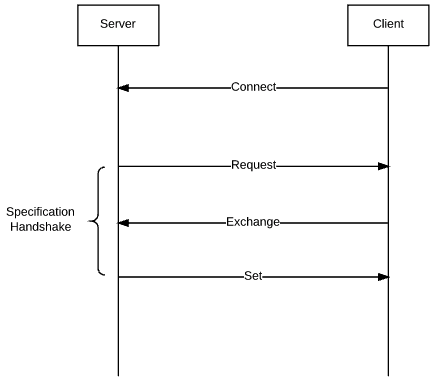
\includegraphics[scale=0.7]{SpecificationHandshake}
\caption{Illustration of Specification Handshake. This handshake is ensure that both client and server use the same specifications for a data transfer.}
\label{fig:specs}
\end{figure}

The packet structures in Figure \ref{fig:specs-struct} correspond to the handshake exchanges in Figure \ref{fig:specs}. The $Request$ message is how the server signals to the client that the server needs to know the specifications of the client. The specifications shared by the client are the ports of the open channels on the client. The client sends this data to the server using the $Exchange$ packet as a header that informs the server of how many port values are being sent. The server uses this exchanged specification to decide how many channels will be used and which ports the client should listen on. When deciding the number of channels, the server will side with the host that supports fewer channels. Once the server decides the specifications the client should use, the server responds with a $Set$ packet followed by the port values the client should use. The client will configure itself to use the channels corresponding to the received ports.

The $Exchange$ and $Set$ packet only express the number of port values that are being sent. The suggested implementation for receiving the port values is to represent port values as 32 bit integers, or 4 bytes, and leverage that fact while reading each port off of the stream. A more optimal approach is to calculate the payload size using the value from the packet header and the size of a port to read in all ports at once.

\begin{figure}[ht]
\centering
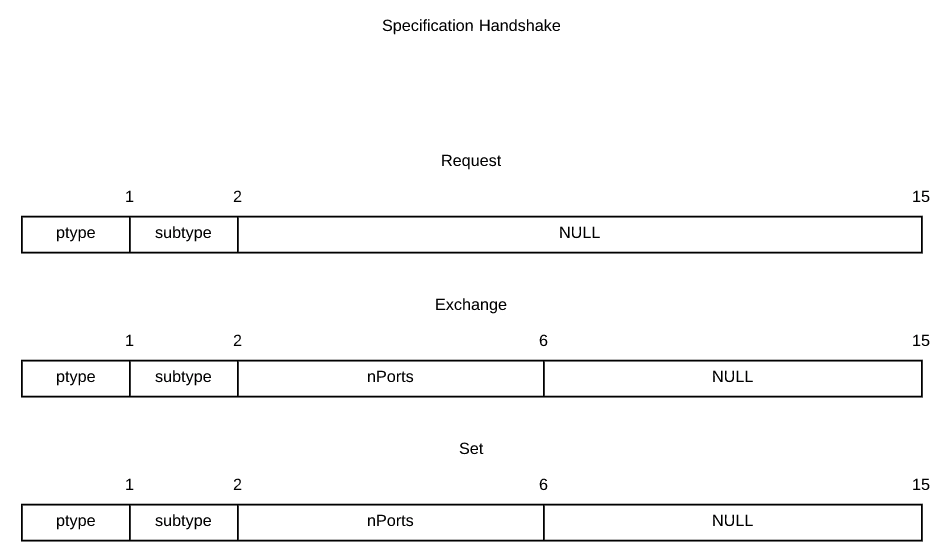
\includegraphics[scale=0.4]{SpecificationHandshakePacketStructures}
\caption{Packet Structure of Specification Handshake. The fields $ptype$ and $subtype$ are for identifying packets. The values of these fields are an implementation detail.}
\label{fig:specs-struct}
\end{figure}

\subsubsection{FTP Handshake}\label{subsec:ftp-hs}

Prior to transferring a file, MCDTP performs another handshake that is similar in design to the specification handshake, as can be seen in Figure \ref{fig:ftp-hs}.

\begin{figure}[ht]
\centering
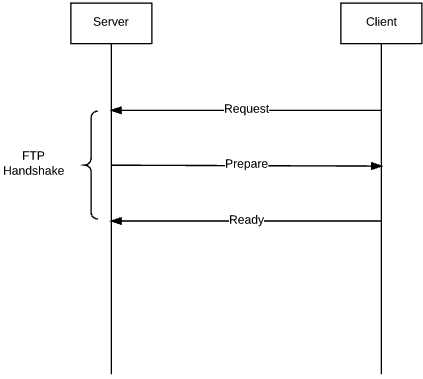
\includegraphics[scale=0.7]{FTPHandshake}
\caption{Illustration of FTP Handshake}
\label{fig:ftp-hs}
\end{figure}

This handshake acts as a concrete step before the data transmission phase and is minimal in design and purpose. This step is so that any asynchronous work that needs to be done first can finish as well as ensure both client and server are prepared for the data transmission phase, which is more of an implementation discussion and will be further discussed in Chapter \ref{chp:impl}. Figure \ref{fig:ftp-struct} is an illustration of the structure of each message in the handshake.

\begin{figure}[ht]
\centering
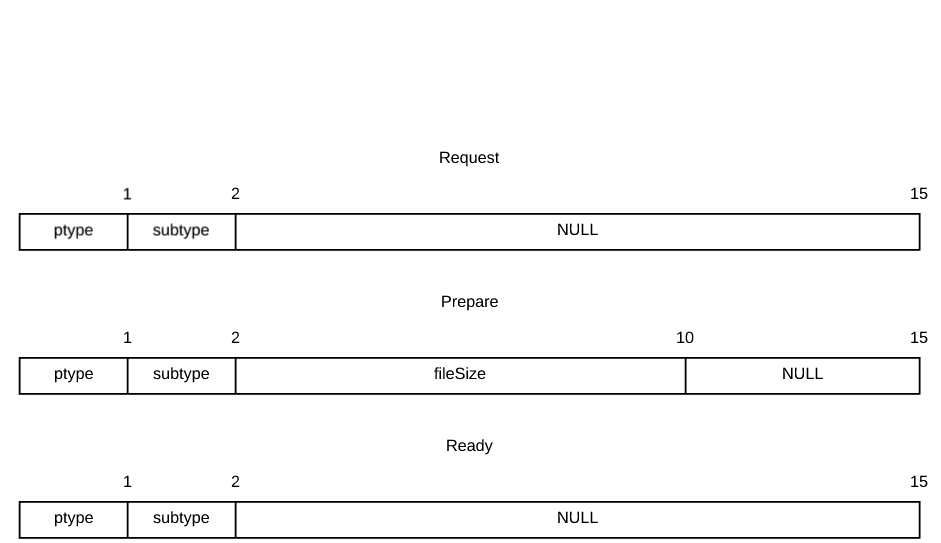
\includegraphics[scale=0.4]{FTPHandshakePacketStructures}
\caption{Packet Structure of FTP Handshake. The fields $ptype$ and $subtype$ are for identifying packets. The values of these fields are an implementation detail.}
\label{fig:ftp-struct}
\end{figure}

 The only information exchanged in this handshake is the size of the file that will be transferred, from server to client. Note that handling file selection has been omitted and will be further discussed in Chapter \ref{chp:c-fw}. Once the client is prepared for transfer and has signaled the server that it is ready, both hosts begin the data transmission phase of the MCDTP protocol.

\subsection{Data Transmission}

The data transmission phase is the second phase in the MCDTP protocol and is comprised mostly of the transmission of a file using the data channels setup in phase 1. The upper portion of Figure \ref{fig:data-tr} illustrates the communication between server and client. The packet retransmission phase and this phase have slight overlap, which is further discussed in Section \ref{subsec:pack-retr}.

\begin{figure}[ht]
\centering
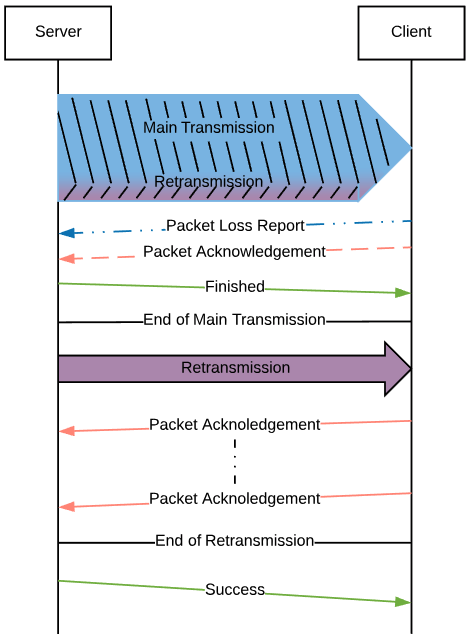
\includegraphics[scale=0.5]{DataTransfer}
\caption{Illustration of Data Transfer\\
The large arrow from server to client at the top represents the data flow for a single channel. The blue in this representation symbolizes the transmission of the file \cite{Meiss2007,He2002,gu2007udt,Fan2010,Aspera2016}.}
\label{fig:data-tr}
\end{figure}

The packet structure of the data transmitted over each channel is shown in Figure \ref{fig:data-tr-struct}. Note that the packet size is not definitively set. As stated previously, the packet size can range from $13B \leq size \leq 64KB$ and is something that needs to be set at an implementation level. The packet header fields ``seqNum'' and ``dLen'' are information regarding the payload of the UDP packet. The ``seqNum'' field is the position in file that the data should be written to. For the sake of being lean, the ``dLen'' field can be used to determine how much of the received payload is file data. This enables the implementation to read in a fixed amount of data. The ``flag'' field acts as a control flag. When the control flag is 0, the packet is a regular packet. A retransmitted packet has a flag value of 1 and 2 is to signal to the client that the channel is switching to the packet retransmission phase. The final packet is illustrated by the green communication line labeled ``Finished'' in Figure \ref{fig:data-tr}, which is sent over the UDP channel.

\begin{figure}[ht]
\centering
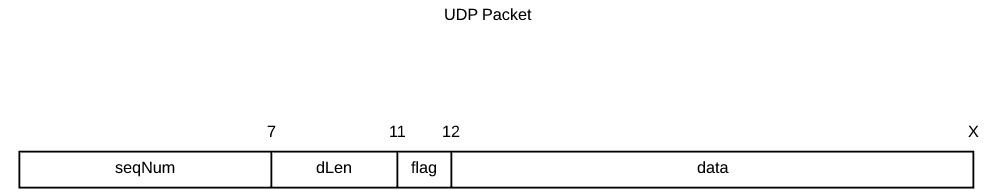
\includegraphics[scale=0.4]{DataTransferPacketStructure}
\caption{Packet Structure of Data Transfer (UDP Packet). The packet is variable in size.}
\label{fig:data-tr-struct}
\end{figure}

As previously mentioned, MCDTP is an experimental protocol. The experimental component attempts to perform a file transfer without the use of congestion control. The protocol tries to exploit the common operating system behavior that when a socket is created, it is given its own receive buffer. With each channel getting its own receive buffer, there is more space to hold incoming packets giving opportunity for handling more data at the Application layer.

\subsection{Packet Retransmission}\label{subsec:pack-retr}

The packet retransmission phase is capable of starting during the data transmission phase. The purpose of this is to recover packets along the way to minimize the duration of this phase and ultimately achieve a successful transfer faster. As can be seen in Figure \ref{fig:data-tr}, retransmission consumes a small portion of bandwidth so as not to impede upon the main transmission during the data transmission phase. The dashed communication lines labeled ``Packet Loss Report'' and ``Packet Acknowledgement'', which share the same structure as is evident in Figure \ref{fig:pack-rec-struct}, only occur when packet loss or packet recovery is detected and are sent over the TCP socket. The values for ``ptype'' and ``subtype'' are as follows:  Packet Loss Report) ``ptype'' = `t', ``subtype'' = `l' and Packet Acknowledgement) ``ptype'' = `t', ``subtype'' = `a'. Since the number of data channels is determined by the implementation, MCDTP uses the ``seqNum'' field to identify the UDP packet the message is in regards to and the ``port'' field to identify which channel the UDP packet was transferred over.

\begin{figure}[ht]
\centering
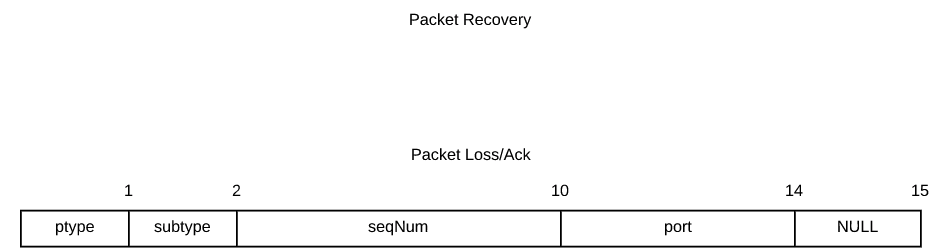
\includegraphics[scale=0.4]{PacketRecoveryStructure}
\caption{Packet Loss and Ack Report Structure for Packet Recovery}
\label{fig:pack-rec-struct}
\end{figure}

After the data transmission phase finishes, the packet retransmission phase is able to consume more bandwidth. The server will send a ``Finished'' packet to signal the client that the data channel on the server has transitioned to the retransmission phase, as illustrated in Figure \ref{fig:data-tr}. As previously mentioned, the control flag in the UDP packet has the value 2. This packet is placed at the head of the retransmission queue in order and is retransmitted until the client acknowledges the packet. This ensures that the server and client are both in the retransmission phase.

\begin{figure}[ht]
\centering
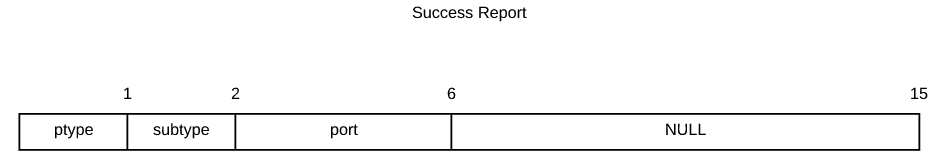
\includegraphics[scale=0.4]{SuccessPacketStructure}
\caption{Packet Structure of Success Report}
\label{fig:success-struct}
\end{figure}

Like RBUDP \cite{He2002}, a channel will continue this phase until the server has received an acknowledgement for all packets that are in recovery for that channel. Once all packets have been received, the server sends a success report, Figure \ref{fig:success-struct}, over TCP thus concluding the work the channel specified by the ``port'' field. The ``ptype'' and ``subtype'' in the success report are set to `t' and `S', respectively. Once all channels have succeeded, the session between the client and server is concluded.